
% X, Y, PRINTNAME, LABEL
\newcommand\petritrans[4]{
    \node[rectangle, draw, color=black, fill=gray, thick, inner sep=0pt, minimum width=0.2cm, minimum height=1cm] (#4) at (#1,#2) {};
    \draw (#1,#2+0.8) node {#3};
}

% X, Y, PRINTNAME, LABEL, INSIDESTUFF
\newcommand\petrinode[5]{
    \node[circle, draw, color=black, thick, inner sep=0pt, minimum size=1cm] (#4) at (#1,#2) { #5 };
    \draw (#1,#2+0.8) node {#3};
}

% X, Y
\newcommand\petrijeton[2]{
    \node[circle, draw,  color=black, fill=gray, thick, inner sep=0pt, minimum size=0.2cm] (test) at (#1,#2) {};
}

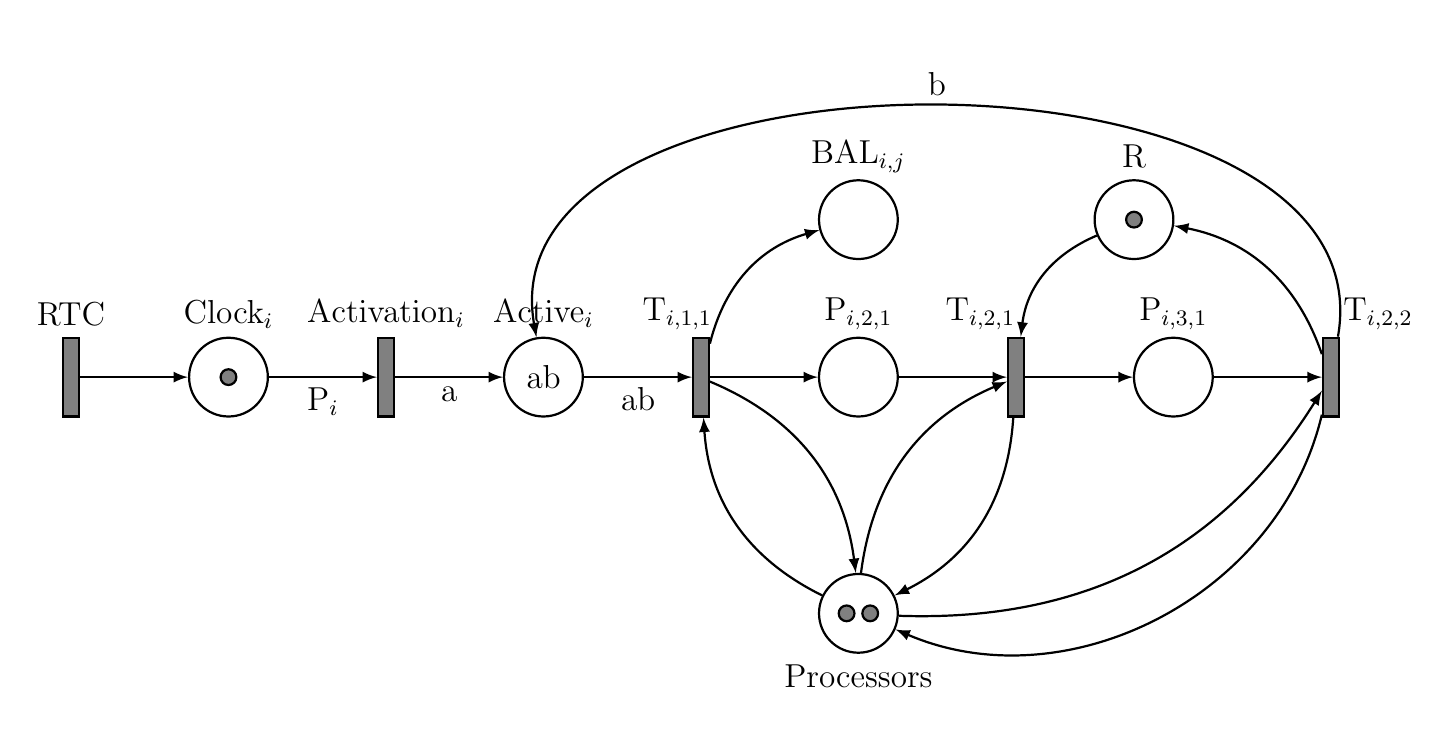
\begin{tikzpicture}[font={\fontsize{12pt}{12}\selectfont}]

    \petritrans{0}{0}{RTC}{rtc}
    \petrinode{2}{0}{Clock$_i$}{clk}{}
    \petrijeton{2}{0}

    \petritrans{4}{0}{Activation$_i$}{activation}
    \petrinode{6}{0}{Active$_i$}{active}{ab}
    
    \petritrans{8}{0}{T$_{i,1,1}$\hspace{0.6cm} }{Ti11}
    \petrinode{10}{0}{P$_{i,2,1}$}{Pi21}{}
    
    \node[circle, draw, color=black, thick, inner sep=0pt, minimum size=1cm] (procs) at (10,-3) {  };
    \draw (10,-3.8) node {Processors};
    \petrijeton{9.85}{-3}
    \petrijeton{10.15}{-3}
    
    \petrinode{10}{2}{BAL$_{i,j}$}{BALij}{}


    \petritrans{12}{0}{T$_{i,2,1}$\hspace{0.9cm} }{Ti21}
    \petrinode{14}{0}{P$_{i,3,1}$}{Pi31}{}
    
    \petrinode{13.5}{2}{R}{R}{}
    \petrijeton{13.5}{2}
    
    
    \petritrans{16}{0}{\hspace{1.2cm}T$_{i,2,2}$}{Ti22}


    \draw[-latex, thick] (rtc) edge node {} (clk);
    \draw[-latex, thick] (clk) edge node[below] {P$_i$} (activation);
    \draw[-latex, thick] (activation) edge node[below] {a} (active);
    \draw[-latex, thick] (active) edge node[below] {ab} (Ti11);
    \draw[-latex, thick] (Ti11) edge node {} (Pi21);
    \draw[-latex, thick] (Pi21) edge node {} (Ti21);
    \draw[-latex, thick] (Ti21) edge node {} (Pi31);
    \draw[-latex, thick] (Pi31) edge node {} (Ti22);
    
    \draw[-latex, thick, bend left] (Ti11) edge node {} (BALij);
    \draw[-latex, thick, bend left] (Ti11) edge node {} (procs);

    \draw[-latex, thick, bend left] (Ti21) edge node {} (procs);


    \draw[-latex, thick, bend right] (Ti22) edge node {} (R);
    \draw[-latex, thick, bend right=100, above] (Ti22) edge node {b} (active);
    \draw[-latex, thick, bend left=50] (Ti22) edge node {} (procs);

    \draw[-latex, thick, bend right] (R) edge node {} (Ti21);
    
    \draw[-latex, thick, bend left] (procs) edge node {} (Ti11);
    \draw[-latex, thick, bend left] (procs) edge node {} (Ti21);
    \draw[-latex, thick, bend right=30] (procs) edge node {} (Ti22);
\end{tikzpicture}
